\documentclass[a4paper,12pt]{article}

\usepackage{amsmath,amssymb,amsthm,multicol,tikz,enumitem}
\usepackage{hyperref}
\usepackage[margin=2cm]{geometry}
\usepackage{fancyvrb}
\usetikzlibrary{calc}
\usepackage{xcolor}

\newcommand\N{\mathbf{N}}
\newcommand\Q{\mathbf{Q}}
\newcommand\R{\mathbf{R}}
\newcommand\Z{\mathbf{Z}}

\newcommand\rem{\textup{rem}}

% Comment out one or the other

%\newcommand\answer[1]{}
%\newcommand\ans[1]{}
%\newcommand\anscommand[1]{}
\newcommand\answer[1]{${}$\\[5pt]{\color{blue}{#1}}\hfill{\color{blue}$\qed$}\\[-5pt]} 
\newcommand\ans[1]{{\color{blue}{#1}}}
\newcommand\anscommand[1]{#1}


\begin{document}

\begin{center}
{\bf\Huge Exam 1, var.2} \\[5pt]
Data Structures \\
Thursday, December 9, 2021\\[5pt]
\textit{*You must justify all your answers to recieve full credit*}
\end{center}

\hrule
\vspace{2pt}
\hrule
\vspace{12pt}

% 1. C++ apart from Object Orientation
% 1.A. Restore/drop parentheses, use syntax trees.
% 1.B. Translate between flowcharts and C++ control structures. 
% 1.C. Use bit arithmetic.
% 1.D. Side-effects in operators, arrays, short-circuit Boolean evaluation.
% 1.E. Run pseudocode pointer operations, draw arrows.
% 1.F. (C++ code) Perform bit manipulation.
% 1.G. (C++ code) Manipulate arrays, char arrays (C-strings), 2D arrays.
% 1.H. (C++ code) Input data using "iostream", "sstream", "getLine", "get", "peek"

% 2. C++ with Object Orientation
% 2.A. Parameter passing to functions, "const" modifier, default parameters.
% 2.B. The order how constructors and destructors are executed.
% 2.C. (C++ code) Implement inheritance with virtual/non-virtual functions.
% 2.D. (C++ code) Custom comparison function to generic sorting, max or similar algorithm.

% 3. Big-O, Omega, Theta Notation
% 3.A. Find the asymptotic growth for a given function.
% 3.B. Compare classes of function growth or order them.
% 3.C. Express time complexity for recursively defined functions. 
% 3.D. Express time complexity for a code snippet ``from the inside out''. 
% 3.E. Find the amortized time complexity for an operation on a given data structure.
% 3.F. Count the number of calls for comparisons or similar functions.

% 4. Lists, stacks, queues.} 
% 4.A. Use Abstract Data Type (ADT) to write algorithms.
% 4.B. (C++ code) Use STL classes for lists, stacks, queues with iterators.


% "1C" "1E" "2B" "3A" "4B" 


\begin{enumerate}

%%%%%%%%
%% 01 %%
%%%%%%%%
\item 
% 1.C. Use bit arithmetic.

\begin{enumerate}
\item Write the right-rotate of the number $216$ by three bits (denoted as $216 >>> 3$). 
Namely, write down $216$ in binary and shift all bits to the right by three positions. 
Show the bit sequence or hexadecimal notation (and also the numeric result). 
Represent all numbers as C++ {\tt int} type (4-byte integers). 
\item Write the XOR result between two numbers: $A = 216$ and $B = 63$. 
(In C++ XOR it is written as carret symbol, but in mathematics is written as $A \oplus B$.)
\end{enumerate}

{\bf Note.} Bit rotation means that all the bits that are shifted out on the right side 
are shifted back in from the left side.


\answer{

{\bf (A)} We can represent $216_{10}$ as $128 + 64 + 16 + 8$, which can be rewritten 
in binary as $\mathtt{11011000}_2$. It takes eight bits (one byte). Since it is a 4-byte integer, we need to precede 
it with three more bytes filled with 0-bits: 

\[ 00000000.00000000.00000000.11011000. \]

(In this notation dots are used just to separate bytes.) After shifting three positions to the right we get: 

\[ 00000000.00000000.00000000.00011011. \]

This number in decimal is $16 + 8 + 2 + 1 = 27$. 

{\bf (B)} The number $216$ was converted to binary in the previous exercise.
The number $63 = 2^6 - 1$ is just multiple 0s followed by six 1s.
Write them one under another (and apply bitwise XOR). 


{\tt 00000000.00000000.00000000.11011000}\\
{\tt 00000000.00000000.00000000.00111111}\\
{\tt ------------------------------------- (XOR)}\\
{\tt 00000000.00000000.00000000.11100111}

The number that was obtained during the last operation is $128 + 64 + 32 + 4 + 2 + 1 = 231$. 

If you wish, you can also compute this from Python command-line: 

\begin{center}
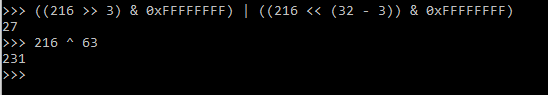
\includegraphics[width=4.5in]{ds-exam1/bit-arithmetic-python.png}
\end{center}
}


%\clearpage

%%%%%%%%
%% 02 %%
%%%%%%%%
\item 
% 1.E. Run pseudocode pointer operations, draw arrows.

The multiplication $C$ of two matrices $A$ and $B$ is defined in \url{https://bit.ly/3lPSWqy}. 
Assume that both matrices are $n \times n$. Then the formula to multiply them becomes:

\[ \mathbf{C}=\begin{pmatrix}
 a_{11}b_{11} +\cdots + a_{1n}b_{n1} & a_{11}b_{12} +\cdots + a_{1n}b_{n2} & \cdots & a_{11}b_{1n} +\cdots + a_{1n}b_{nn} \\
 a_{21}b_{11} +\cdots + a_{2n}b_{n1} & a_{21}b_{12} +\cdots + a_{2n}b_{n2} & \cdots & a_{21}b_{1n} +\cdots + a_{2n}b_{nn} \\
\vdots & \vdots & \ddots & \vdots \\
 a_{n1}b_{11} +\cdots + a_{nn}b_{n1} & a_{n1}b_{12} +\cdots + a_{nn}b_{n2} & \cdots & a_{n1}b_{1n} +\cdots + a_{nn}b_{nn} \\
\end{pmatrix} 
\]

{\bf (A)} Find the worst-case time complexity to multiply two $n \times n$ matrices, if any multiplication of 
two numbers and any addition of two numbers takes constant time $O(1)$.\\
{\bf (B)} Now assume that the numbers in matrices are very long -- each number is $m$ bits long. 
What is the worst-case time complexity to multiply two $n \times n$ matrices, if 
any multiplication of two numbers has time complexity $O(m^2)$, but any addition has time complexity $O(m)$? 

\answer{

{\bf (A)} The time complexity to multiply two matrices by the above formula is $O(n^3)$ -- 
one needs to compute exactly $n^2$ entries. And for each entry there are $n$ multiplications and 
$n-1$ additions (total number of arithmetic operations is $n + (n-1) = 2n-1$). 
And we can see that $n^2 (n - 1)$ is in $O(n^3)$. 

{\bf (B)} Once again there are $n^2$ entries to compute. But now we have $n$ multiplications per entry, 
and each multiplication costs $O(m^2)$. (There are additions as well, but additions are
faster than multiplications so they are not counted.) So the time needed for a single 
entry of the product matrix is $n \cdot m^2$.

For the whole matrix multiplication the time complexity is $n^2 \cdot (n \cdot m^2)$, which 
is in $O(n^3 m^2)$. 

{\bf Note.} Both $m$ and $n$ should be in the answer -- as one of the numbers can be much larger
than the other one. Therefore, the answer should not be simplified to $O(m^5)$ or $O(n^5)$
(as the length of individual numbers $m$ has nothing to do with the size of the matrix $n$).
}






%%%%%%%%
%% 03 %%
%%%%%%%%
\item \label{q:q4}
% 4.B. (C++ code) Use STL classes for lists, stacks, queues with iterators.

The following C++ program declares a class {\tt Pair}. 
Pairs are {\em lexicographically ordered}: 
\[
(x_1, y_1) < (x_2, y_2)\ \ \text{iff}\ \ x_1 < x_2\ \vee\ (x_1 = x_2\ \wedge\ y_1 < y_2).
\]
Complete the code below so that, when compiled and executed, in order:
\begin{itemize}
\item a positive integer $n$ is input,
\item $n$ pairs from the standard input are input,
\item the $n$ pairs are pushed on the stack, skipping pairs which are not lexicographically larger than the current top element of the stack,
\item the remaining pairs are output to the standard output as separate lines in their original order.
\end{itemize}

Use the overloaded operators ``{\tt cout << pair}'', ``{\tt cin >> pair}'', ``{\tt p1 < p2}''
for input, output and comparisons. The only data structure to use is STL stack. 
If necessary, you may use several stacks.

\begin{Verbatim}[frame=single,numbers=left]
#include <iostream>
#include <stack>
using namespace std;
class Pair { public: int x; int y; }; 
istream &operator>>(istream  &input, Pair &p ) { 
  input >> p.x >> p.y;   return input;            
}
ostream &operator<<(ostream &output, const Pair &p ) { 
  output << "(" << p.x << "," << p.y << ")";   return output;            
}
bool operator<(const Pair &left, const Pair &right) {
  // implement the lexicographic comparison operator.
}
int main() {
  // Input the total number of pairs, then 2*n integers (the pairs). 
  // Output those pairs which are in lexicographically increasing order.
}
\end{Verbatim}

{\bf Sample input}

\begin{Verbatim}[frame=single]
5
4 17
4 17
5 1000
7 12
7 9
\end{Verbatim}

{\bf Sample output}

\begin{Verbatim}[frame=single]
(4,17)
(5,1000)
(7,12)
\end{Verbatim}



\answer{
One possible solution is shown below. 
}

{\small
\begin{Verbatim}[frame=single,numbers=left]
#include <iostream>
#include <stack>
using namespace std;
class Pair { 
  public: int x; int y; 
  Pair() { 
    cout << "Default constructor" << endl; 
  }
  Pair(const Pair& arg) { 
    cout << "Copy constructor on (" << x << "," << y << ")" << endl; 
    x = arg.x;
    y = arg.y;
  }
  ~Pair() {
    cout << "Destructor on (" << x << "," << y << ")" << endl; 
  }

}; 
istream &operator>>(istream  &input, Pair &p ) { 
  input >> p.x >> p.y;   return input;            
}
ostream &operator<<(ostream &output, const Pair &p ) { 
  output << "(" << p.x << "," << p.y << ")";   return output;            
}
bool operator<(const Pair &left, const Pair &right) {
  return (left.x < right.x) || (left.x == right.x && left.y < right.y);
}
int main() {
    int n; 
    cin >> n; 
    stack<Pair> myStack;
    for (int i = 0; i < n; i++) {
        Pair p; 
        cin >> p;
        if (myStack.empty() || myStack.top() < p) {
            myStack.push(p);
        }        
    }
    stack<Pair> otherStack;
    while (!myStack.empty()) {
        otherStack.push(myStack.top());
        myStack.pop();
    }    

    while (!otherStack.empty()) {
        cout << otherStack.top() << endl;
        otherStack.pop();
    }    
}
\end{Verbatim}
}



\clearpage


%%%%%%%%
%% 04 %%
%%%%%%%%
\item 
Consider two functions: $f(n) = 3^n$ and $g(n) = n!$. 

{\bf (A)} Is $f(n)$ in $O(g(n))$?\\
{\bf (B)} Is $g(n)$ in $O(f(n))$?

In both cases justify your answer by using the definition of Big-O Notation. 

{\bf The Definition of Big-O:} 
Let $f$ and $g$ be functions from positive integers to positive real numbers.  
One writes $f(x) = O( g(x))$
if the absolute value of $f(x)$ does not exceed $M|g(x)|$ for some constant $M$ and all sufficiently 
large $x \geq x_0$. 


\answer{

{\bf (A)} Yes, $3^n$ is in $O(n!)$. 

Verify by the definition: Take $M = 1$ and $x_0 = 7$. We have the following inequality: 

\[ f(7) = 3^7 = 2187 < g(7) = 7! = 5040. \]

Inequality $f(x) < g(x)$ will also hold for all values $x > 7$. The left side ($f(x) = 3^x$) 
increases only $3$ times as you replace $x$ by $x+1$, since $3^{x+1} = 3 \cdot 3^x$. 
On the other hand, function $g(x + 1) = (x+1)! = (x+1) \cdot x! = (x+1) g(x)$ increases 
$x+1$ times as you replace $x$ by $x+1$. And we must have $x+1 > 3$ for all values of $x$ that are larger than $7$.

{\bf (B)} No, $n!$ is not in $O(3^n)$. 

Assume from the contrary that there exists $M$ and $x_0$ such that 
for all $x \geq x_0$ the inequality $n! \leq M \cdot 3^n$ must hold as soon as $n \geq x_0$. 

We want to get a contradiction. Pick some value $N$ such that $N > x_0$ and $N > 4$. 
Denote the ratio of both sides of inequality: 

\[ \frac{g(N)}{M \cdot f(N)} = \frac{N!}{M \cdot 3^N} = R. \]

Accordingly to the assumption $R < 1$, and also for all $x > N$ we must have $\frac{g(x)}{M \cdot f(x)} < 1$. 
Pick value $D$ such that ${\displaystyle \left( \frac{4}{3} \right)^D > \frac{1}{R}}$. 
It must exist as $4/3 > 1$, so the powers will ultimately exceed any positive number, no matter how large. 

Once we pick $x = N + D$, we have $\frac{x!}{M \cdot 3^x}$ will grow larger than $1$, since 
every factor $\frac{N+1}{3}>\frac{4}{3}, \frac{N+2}{3}>\frac{4}{3}, \ldots, \frac{N+D}{3}>\frac{4}{3}$. 

Thus $\frac{g(x)}{M \cdot f(x)} > 1$, which contradicts the definition of Big-O. 
}


\clearpage

%%%%%%%%
%% 05 %%
%%%%%%%%
\item
Assume that you have a stack data structure (you can create empty stack, push and pop any elements, and look at the
top element). 
Write pseudocode that rotates the items in the stack so that the topmost element goes to the very bottom. 
(Note: You can use as many stack data structures as you need.)

\begin{verbatim}
apple                         banana
banana    ===rotate==>        cucumber
cucumber                      apple
\end{verbatim}

\answer{

We implement function $\text{\sc RotateStack}(S_1)$ that will rotate the stack. 
We will also use two auxiliary stacks $S_2$ and $S_3$ that are initially empty. 

\begin{enumerate}[label={\arabic*.}]
\item {\bf if} $S_1.empty()$ 
\item \mbox{}\hspace{2em}{\bf return} $S_1$
\item $S_2 = emptyStack()$\hspace{2em} {\em (this stack will be used to reverse $S_1$)}
\item $S_3 = emptyStack()$\hspace{2em} {\em (this stack will be used to return the result)}
\item $topValue = S_1.top()$\hspace{2em} {\em (store the value at the top)}
\item $S_1.pop()$\hspace{2em} {\em (remove the top element)}
\item {\bf while not} $S_1.empty()$\hspace{2em} {\em (this loop reverses $S_1$ and inserts into $S_2$)}
\item \mbox{}\hspace{2em} $elem = S_1.top()$
\item \mbox{}\hspace{2em} $S_1.pop()$
\item \mbox{}\hspace{2em} $S_2.push(elem)$
\item $S_3.push(topValue)$ \hspace{2em} {\em (the top element of $S_1$ goes into $S_3$ first)}
\item {\bf while not} $S_2.empty()$ \hspace{2em} {\em (this loop reverses $S_2$ again to preserve order)}
\item \mbox{}\hspace{2em} $elem = S_2.top()$
\item \mbox{}\hspace{2em} $S_2.pop()$
\item \mbox{}\hspace{2em} $S_3.push(elem)$
\item {\bf return} $S_3$ 
\end{enumerate}
}




\end{enumerate}


\end{document}